\begin{center} % Tittelen på dokumentet, sentrert, stor og i bold skrift
\LARGE{\textbf{Eksperiment 4 - Substitusjonsreaksjoner. Alkylhalider.}}
\end{center}
[Alt som står i firkantklammer er instruksjoner/kommentarer som skal fjernes, eller erstattes, unntatt enhetene i datatabeller. Se ellers vedlegg i oppgaveheftet for organisk-lab om oppsett av rapport.]
\section*{Sammendrag}

\section{Teori}


\subsection{Reaksjonsligninger}

\subsubsection{\texorpdfstring{S\textsubscript{N}2}r reaksjoner}

\begin{equation}
	\begin{aligned}
		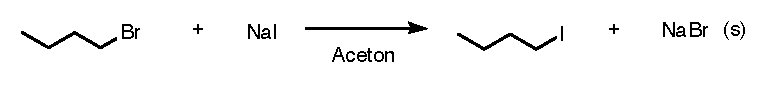
\includegraphics[scale=0.9]{Figurer/Sn2-1.eps}
	\end{aligned}
	\label{eq:SN2-1}
\end{equation}

\begin{equation}
	\begin{aligned}
		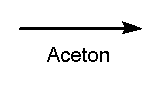
\includegraphics[scale=0.9]{Figurer/Sn2-2.eps}%
	\end{aligned}
	\label{eq:SN2-2}
\end{equation}




\subsubsection{\texorpdfstring{S\textsubscript{N}1}r reaksjoner}

\begin{equation}
	\begin{aligned}
		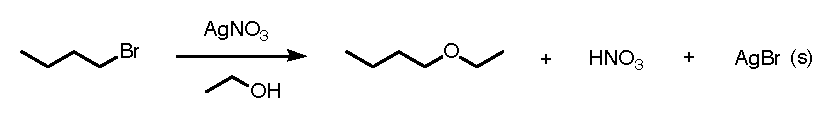
\includegraphics[scale=0.9]{Figurer/Sn1-1.eps}%
	\end{aligned}
	\label{eq:SN1-1}
\end{equation}

\begin{equation}
	\begin{aligned}
		
\includegraphics[scale=0.9]{Figurer/Sn1-2.eps}%
	\end{aligned}
	\label{eq:SN1-2}
\end{equation}


\section{Eksperimentelt og resultater}
Det ble utført 20 reaksjoner, vist i Tabell \ref{tab:iaceton} og Tabell \ref{tab:ietanol}. For alle reaksjonene, unntatt prøve nr. 17 og 18 ble saltløsningen tilsatt først i et reagensrør, og deretter ble alkylhalidet tilsatt. For prøve 17 og 18 var rekkefølgen omvendt.

\begin{sidewaystable}[!htbp]
	\begin{center}
		\caption{Resultater fra \texorpdfstring{S\textsubscript{N}2}r reaksjoner mellom ulike alkylhalider og natriumjodid i aceton}
		\label{tab:iaceton}
		\begin{tabular}{lccl}
			\toprule\\
			Prøve nr. & Alkylhalid & NaI i aceton & Observasjoner\\
			(Lign.) & (kons., volum) & (kons., volum) & \\
			\midrule\\
			1 (\ref{eq:SN2-1}) & 1-brombutan (5 dråper) & 15\%, 5 \si{\milli\liter} & Rask reaksjon, momentant bunnfall.\\
			2 & & & \\
			3 & & & \\
			4 & & & \\
			5 & & & \\
			6 & & & \\
			7 & & & \\
			8 & & & \\
			9 & & & \\
			10 (\ref{eq:SN2-1}) & 1-brombutan (1 M, 5\si{\milli\liter}) & 7.5\%, 5 \si{\milli\liter} & Treg reaksjon, utfelling av [FYLL INN: farge] pulver etter ca. [FYLL INN TID] minutter.\\
			11 & & & \\
			\bottomrule\\
		\end{tabular}
	\end{center}
\end{sidewaystable}


\begin{sidewaystable}[!htbp]
	\begin{center}
		\caption{Resultater fra \texorpdfstring{S\textsubscript{N}1}r reaksjoner mellom ulike alkylhalider og sølvnitrat i etanol}
		\label{tab:ietanol}
		\begin{tabular}{lccl}
			\toprule\\
			Prøve nr. & Alkylhalid & \ce{AgNO3} i etanol & Observasjoner\\
			(Lign.) & (kons., volum) & (kons., volum) & \\
			\midrule\\
			12 \\
			13 \\
			14 \\
			15 \\
			16 \\
			17 \\
			18 \\
			19 \\
			20 \\
			\bottomrule\\
		\end{tabular}
	\end{center}
\end{sidewaystable}

\section{Resultater}

\section{Diskusjon}
